\documentclass{ctexart}
\usepackage{listings}
\usepackage[dvipsnames]{xcolor}
\usepackage{cite}
\usepackage{diagbox}
\usepackage{fancyhdr} % 加载fancyhdr宏包,用于设置页眉和页脚
\pagestyle{fancy} % 设置页面样式
\fancyhf{} % 清除默认的页眉和页脚的内容
\fancyfoot[C]{\thepage} 
\renewcommand{\headrulewidth}{0pt} % 将页眉的横线宽度设置为0pt
\usepackage[left=2.5cm,right=2.5cm,top=2.5cm,bottom=2.5cm]{geometry}

\usepackage{graphicx}
\usepackage{longtable}
\usepackage{tabularx}
\usepackage{float}
\usepackage{amsmath}%引用宏包要放在documentclass后面,否则报错
\usepackage{hyperref}
\usepackage{bm}
\usepackage{amssymb}
\usepackage{esint}
\usepackage{booktabs}
%\usepackage{subfiles}%用于分章节管理引用,使各章节引用来源于各自的文件,编号相互独立
\usepackage{amsthm}
\title{数字电路实验\quad 实验报告}
\author{Your Name}
\date{\today}

\begin{document}
\maketitle
\section{实验内容}
% 用逻辑门实现设计2421BCD码的检测电路:
\begin{enumerate}
    \item 
\end{enumerate}
\section{实验器材}
% Pocketlab、电脑、导线若干、剥线钳、镊子、限流电阻一个、红色LED灯一个、7404芯片一个、7400芯片一个、7420芯片一个。芯片的引脚图如下所示
%三个图片并排
\begin{figure}[H]
    \centering
    \begin{minipage}{0.25\textwidth}
    \centering
           \includegraphics[width=0.8\textwidth]{}
           \caption{}
    \label{}
    \end{minipage}
    \hspace{0.05\textwidth}
    \begin{minipage}{0.25\textwidth}
    \centering
           \includegraphics[width=0.8\textwidth]{}
           \caption{}
    \label{}
    \end{minipage}
     \hspace{0.05\textwidth}
    \begin{minipage}{0.28\textwidth}
    \centering
           \includegraphics[width=0.8\textwidth]{}
           \caption{}
    \label{}
    \end{minipage}
\end{figure}
\section{实验原理}
% 题目要求识别2421BCD码中的伪码,若设输入变量为A,B,C,D,输出为F,并规定伪码输出为1,有效码输出为0,则可以列出如下真值表

\begin{longtable}{|p{2cm}<{\centering}| p{2cm}<{\centering} |p{2cm}<{\centering}| p{2cm}<{\centering} |p{2cm}<{\centering}|}%手动调间距
\caption{真值表}
\hline
  A & B & C & D & F \\
\hline
  0 & 0 & 0 & 0 & 0 \\
\hline
  0 & 0 & 0 & 1 & 0 \\
\hline
  0 & 0 & 1 & 0 & 0 \\
\hline
  0 & 0 & 1 & 1 & 0 \\
\hline
  0 & 1 & 0 & 0 & 0 \\
\hline
  1 & 0 & 1 & 1 & 0 \\
\hline
  1 & 1 & 0 & 0 & 0 \\
\hline
  1 & 1 & 0 & 1 & 0 \\
\hline
  1 & 1 & 1 & 0 & 0 \\
\hline
  1 & 1 & 1 & 1 & 0 \\
\hline
  0 & 1 & 0 & 1 & 1 \\
\hline
  0 & 1 & 1 & 0 & 1 \\
\hline
  0 & 1 & 1 & 1 & 1 \\
\hline
  1 & 0 & 0 & 0 & 1 \\
\hline
  1 & 0 & 0 & 1 & 1 \\
\hline
  1 & 0 & 1 & 0 & 1 \\
\hline
\end{longtable}
对应真值表可以做出卡诺图
\begin{table}[H]
    \centering
    \caption{卡诺图}
    \begin{tabular}{|c|c|c|c|c|}
\hline
\diagbox{AB}{CD} & 00 & 01 & 11 & 10 \\
\hline
00 & 0 & 0 & 0 & 0  \\
\hline
01 & 0 & 1 & 1 & 1  \\
\hline
11 & 0 & 0 & 0 & 0  \\
\hline
10 & 1 & 1 & 0 & 1  \\
\hline
\end{tabular}
    \label{tab:卡诺图}
\end{table}
% 写出逻辑函数的表达式
%连等式的写法
\begin{equation}
    \begin{aligned}
F &=\sum m(5,6,7,8,9,10)\\
&=AB'C'+AB'D'+A'BD+A'BC\\
&=AB'(C'+D')+A'B(C+D)\\   
&=AB'(CD)'+A'B(C'D')'
    \end{aligned}
\end{equation}
\section{电路设计与实现}
\subsection{电路仿真图}
在Multisim中连接好电路仿真图
\begin{figure}[H]
    \centering
    \includegraphics[width=0.75\linewidth]{}
    \caption{}
    \label{}
\end{figure}

\subsection{电路实物图}
按电路仿真图搭好实物电路图
\begin{figure}[H]
    \centering
    \includegraphics[width=0.75\linewidth]{}
    \caption{}
    \label{}
\end{figure}
\section{功能测试}
%逐步测试及其调整
%pockelab、截图要一图一行才看得清楚
如图是Pocketlab逻辑分析仪的部分实验截图
\begin{figure}[H]
    \centering
    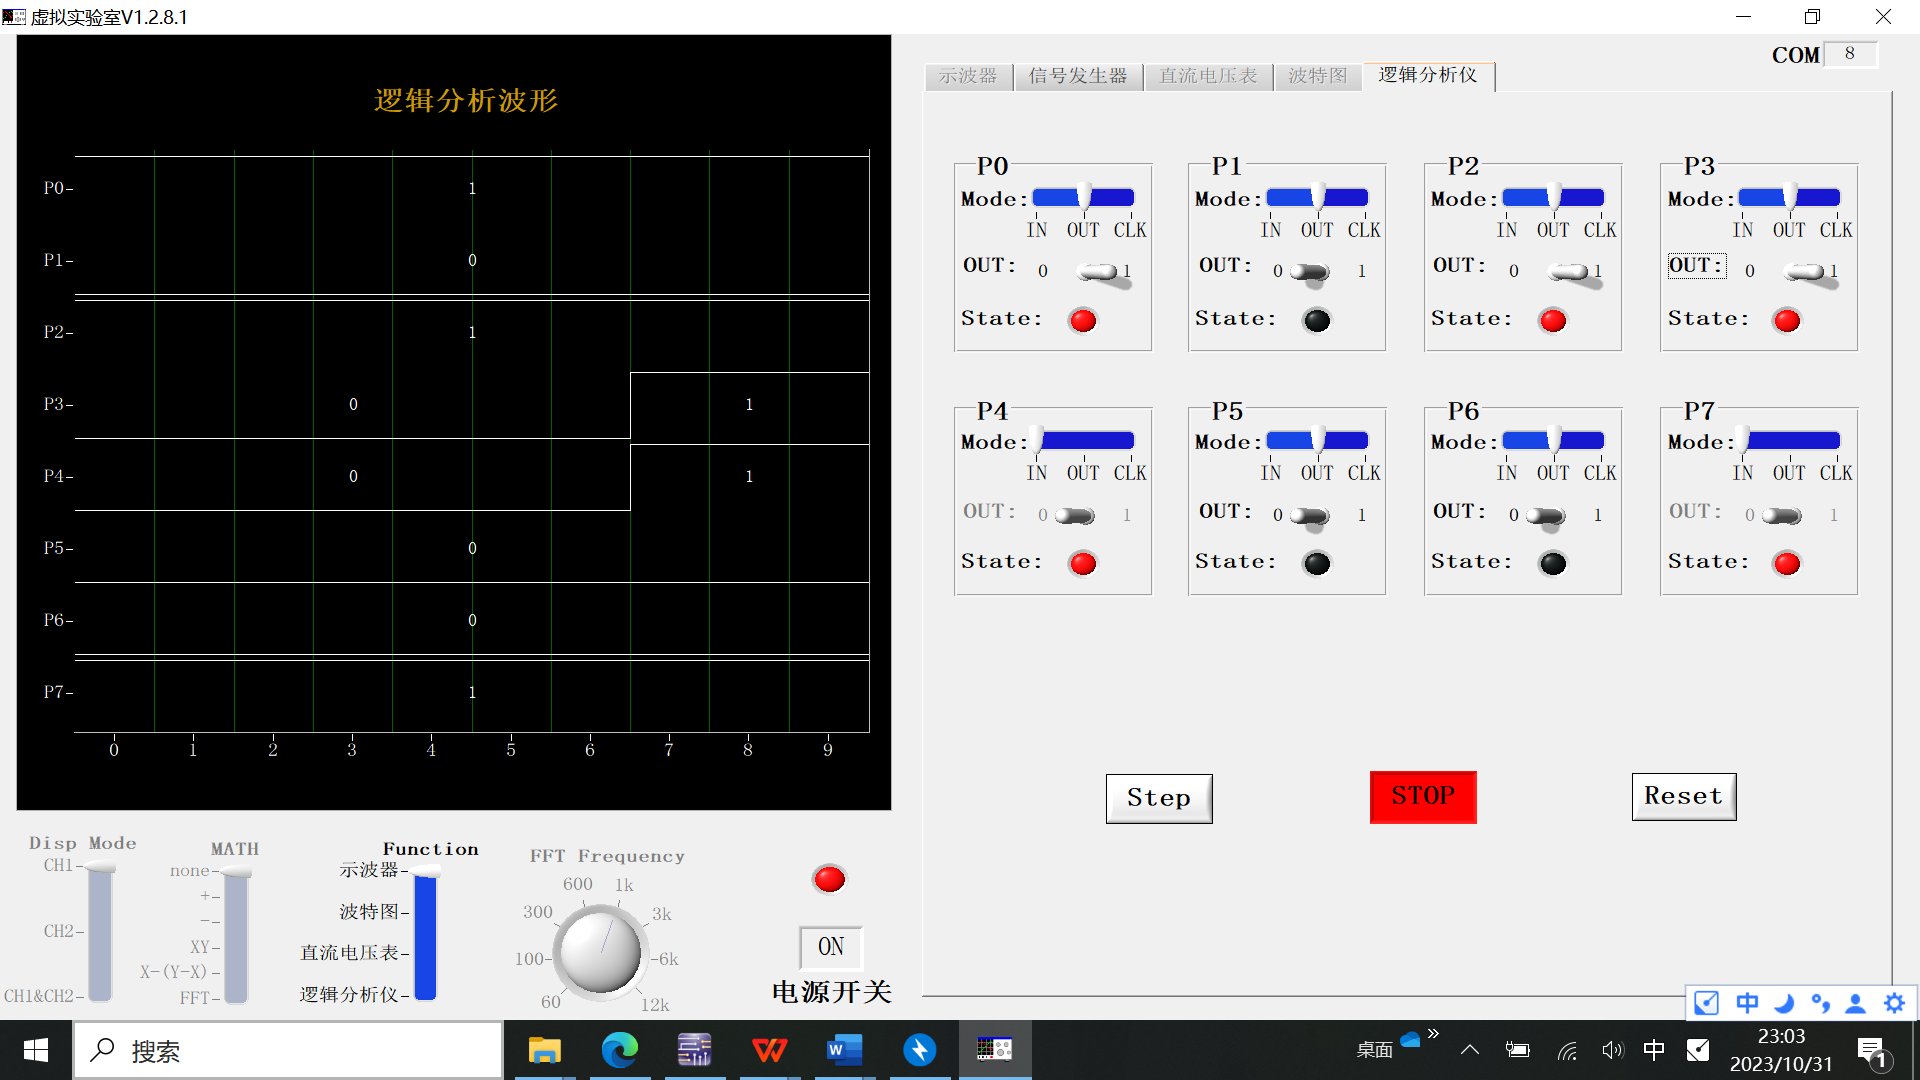
\includegraphics[width=0.75\textwidth]{fig/Pocketlab界面截图1.png}
    \caption{Pocketlab界面截图1}
    \label{Pocketlab界面截图1}
\end{figure}
\begin{figure}[H]
    \centering
    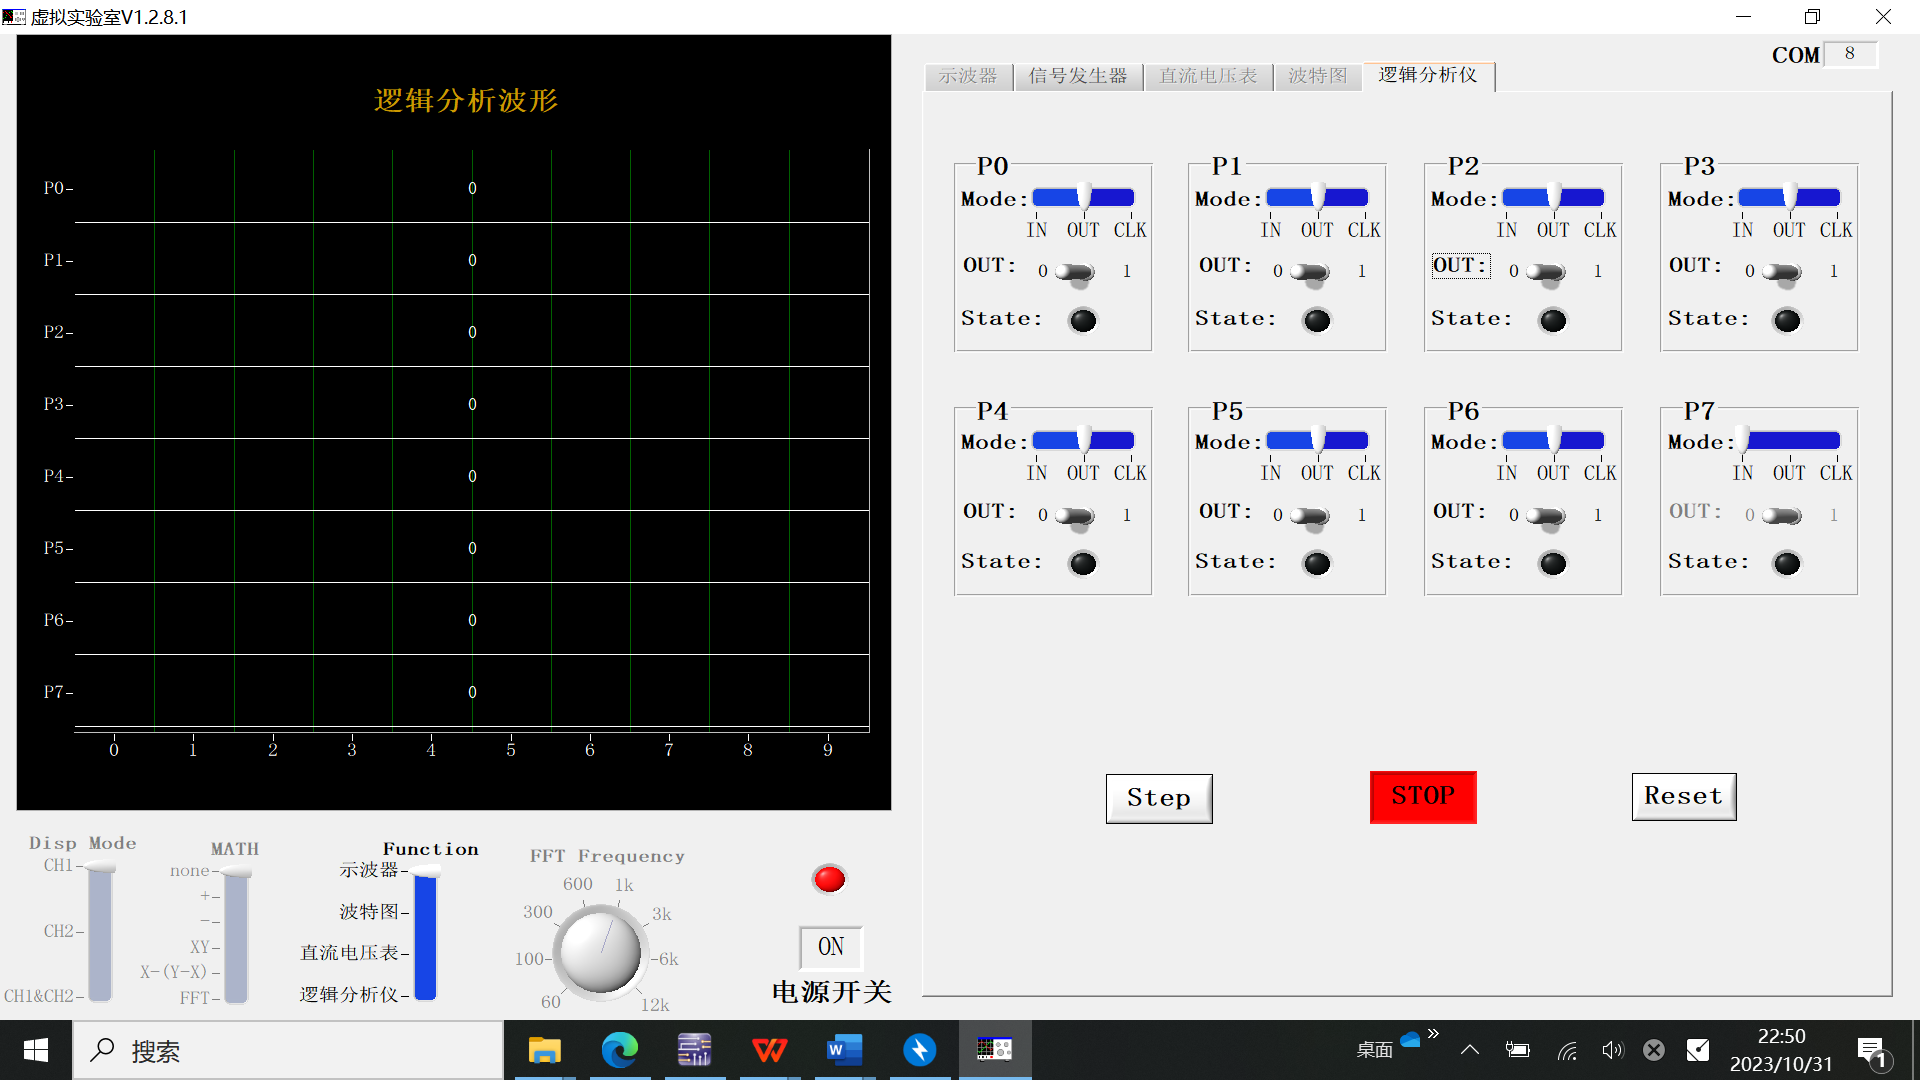
\includegraphics[width=0.75\textwidth]{fig/Pocketlab界面截图2.png}
    \caption{Pocketlab界面截图2}
    \label{Pocketlab界面截图2}
\end{figure}
\section{实验总结与反思}
% 本次实验总体来说较为顺利,需求分析、逻辑表达、电路设计、仿真测试各个环节都没有遇到太大问题。但仍在以下几个方面有待提升
\begin{enumerate}
    \item 
\end{enumerate}

\end{document}